\subsection{Distributed Extent Management System}
\label{sec:cases:azurestore}

We used \psharp to test the \emph{distributed extent management} component of the Windows Azure vNext distributed storage system. This component is responsible for managing the partitioned extent metadata and works as follows.

\subsection{Live Azure Table Migration}

\def\term#1{\emph{#1}}
We also used \psharp to test the MigratingTable library, which is capable of transparently migrating a data set between tables in the Windows Azure storage service while an application is accessing the data set.

\begin{figure}[t]
\centering
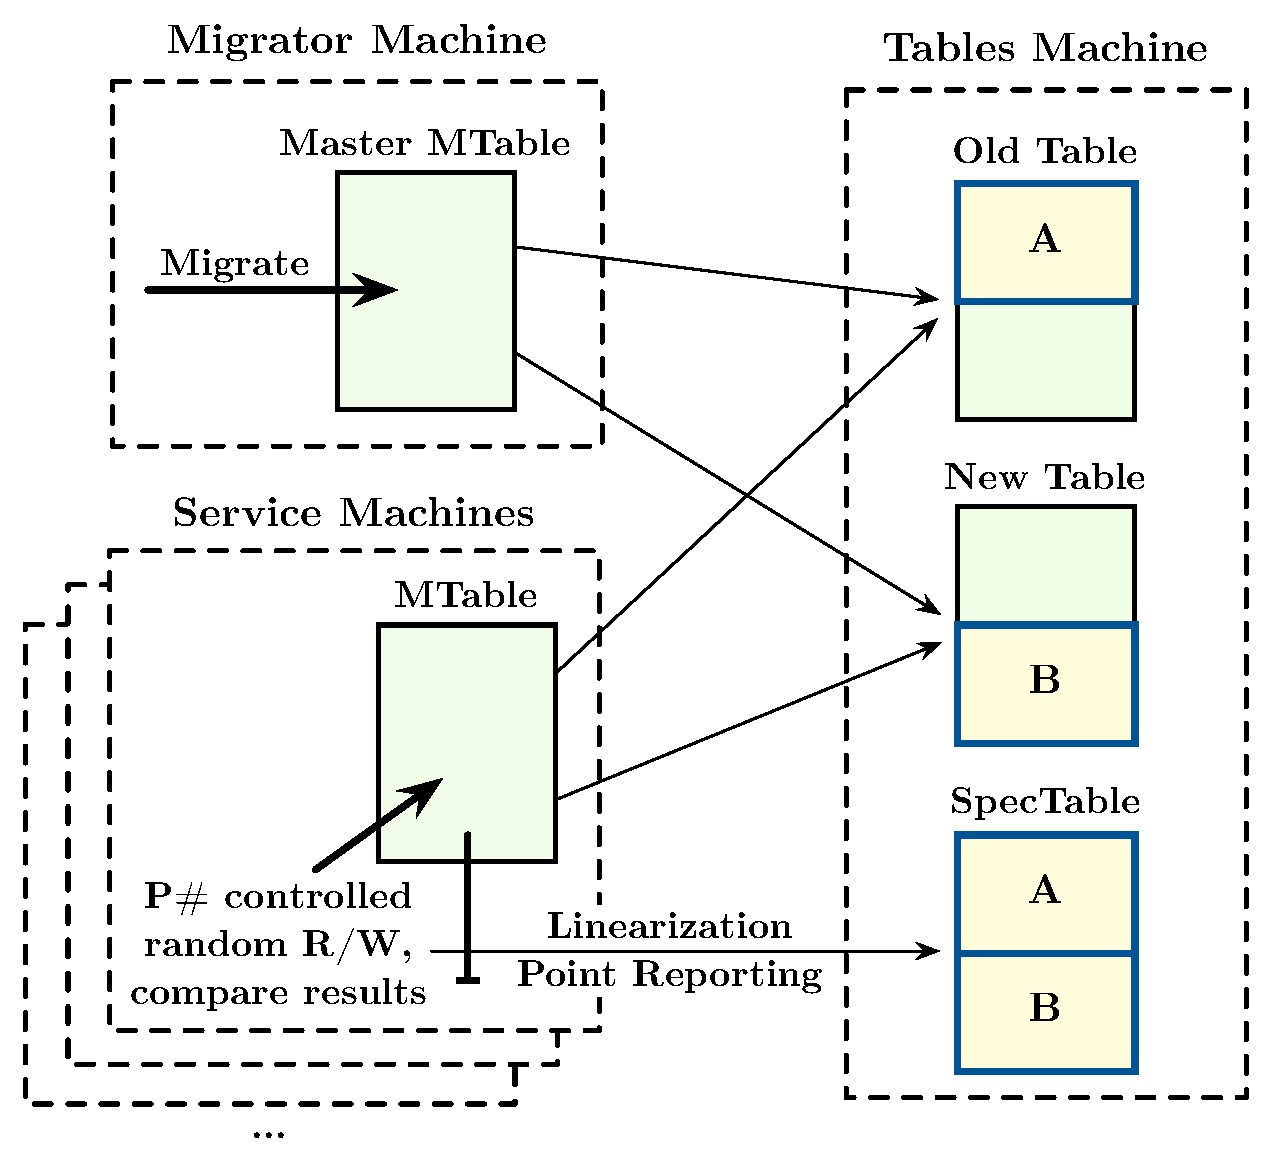
\includegraphics[width=\linewidth]{img/mocked_migration}
\caption{MigratingTable \psharp correctness test environment.}
\label{fig:mockedmigration}
\end{figure}

Since we were designing a new concurrent protocol that we expected to become increasingly complex over time as we add optimizations, we planned from the beginning to maintain a \psharp test harness along with the protocol to maintain confidence in its correctness.

MigratingTable implements an interface called IChainTable2, which provides the core read and write functionality of the original Azure table API with one exception: it provides \term{streaming reads} with a weaker consistency property than multi-page reads in the original API, since the original property would have been difficult to achieve for no benefit to applications we could foresee.  MigratingTable requires that its backend tables also implement IChainTable2, and we wrote a simple adapter to expose physical Azure tables as IChainTable2.  Our goal was then to verify that when multiple application processes issue ``input'' read and write calls to their own MigratingTable instances with the same backend tables, the behavior complies with the specification of IChainTable2 for the combined input history.

\subsubsection{Input generation}

Of course, there are many possible input histories to test.  Since we originally hoped for a comprehensive form of verification and we didn't feel we had good intuition to prepare a set of specific test cases that would make us confident of having caught any and all concurrency bugs in the protocol, it was natural for us to sample from a distribution of input histories that we defined to exercise all the features of IChainTable2 within certain bounds.  Furthermore, it was natural to let \psharp control the choice of input history as well as the machine interleaving so we could reproduce both using a single random seed.

All of our input histories include two application processes.  Each process performs either a single streaming read or a sequence of two atomic calls, each a read or a batch write.  Each batch write call includes one or two operations, where the operation type is chosen from the set supported by IChainTable2 (Insert, Replace, Merge, Delete, InsertOrReplace, InsertOrMerge, DeleteIfExists) and the row key is chosen from $\{0, \ldots, 5\}$.  If the operation requires an If-Match value, it is equally likely to be \texttt{*}, the current ETag of the row (if it exists), or some non-matching value.  Finally, the new entity includes a user-defined property \texttt{isHappy} whose value is equally likely to be true or false.  For both atomic and streaming reads, the filter expression is equally likely to be empty (i.e., match everything), \texttt{isHappy eq true}, or \texttt{isHappy eq false}.

\subsubsection{Model structure}

% N.B. SpecTable = InMemoryTableWithHistory in the current codebase. ~ Matt 2015-08-17
To comprehensively verify the behavior of MigratingTable under an arbitrary input history, we needed some formulation of the IChainTable2 specification to which to compare it.  Since the specification is deterministic under sequential calls except for the results of streaming reads, we decided the easiest approach was to write an in-memory reference implementation called SpecTable.  Given a streaming read call, SpecTable can produce a set of all results that are compliant with the specification.  Our correctness property is then:
% Convert to some theorem-like environment? ~ Matt
\begin{quote}
For every execution trace of a collection of MigratingTables backed by the same pair of \term{old} and \term{new} SpecTables (where \psharp chooses the actual result of each streaming read from the valid set) in parallel with the migrator job, there exists a linearization of the combined input history such that the output in the original trace matches the output of a ``reference'' SpecTable on the linearized input.
\end{quote}
%
We instrumented MigratingTable to report the intended \term{linearization point} of each input call, which in our setting is always one of the corresponding \term{backend calls} to the backend tables (often the last).  Specifically, after each backend call completes, MigratingTable reports whether that call was the linearization point, which may depend on the result of the call.  This makes it possible to verify the correctness property as the model executes.  The model consists of a \psharp \term{tables machine} containing all three SpecTables; a collection of \term{service machines} containing identically configured MigratingTables; and a \term{migrator machine} that performs the background migration (Figure~\ref{fig:mockedmigration}).  Each service machine issues a random sequence of input calls to its MigratingTable, which sends backend calls to the tables machine.  When MigratingTable reports the linearization point of an input call, the service machine sends that input call to the reference table.  When an input call completes, the service machine checks that the results from the MigratingTable and the reference table agree.  \psharp controls the interleaving of the backend calls.  To ensure that the reference table is never observed to be out of sync with the backend tables, after the tables machine processes a backend call, it enters a state that defers further backend calls until MigratingTable has reported whether the backend call was a linearization point and (if so) the call to the reference table has been made.  We use the \psharp random scheduling strategy; we were afraid that an exhaustive strategy would only be feasible within bounds so low that we would miss some bugs.

We wanted to implement the core MigratingTable algorithms in \csharp ``async/await'' code, like most of Artifact Services, to achieve both good readability and good performance.  We used a method similar to that described in Section~\ref{sec:psharp:async} to bring the generated TPL tasks under the control of the \psharp scheduler.  Then we implemented an ``async'' RPC mechanism based on the .NET RealProxy class that automates the generation of proxies for objects hosted by other \psharp machines (in our setting, the service machines use proxies for the SpecTables and various auxiliary objects hosted by the tables machine).  When a machine calls a method on a proxy, the proxy sends a \psharp message to the host machine, causing it to execute the method call on the original object and send back the result, which the proxy then returns.  Thus, the use of these proxies as IChainTable2 backends is transparent to the MigratingTable library, thanks to dynamic dispatch.

